\newpage
\section{ワイヤ駆動式魚ロボットの開発}
\subsection{本研究の目的}
初めに,本研究の目的について述べる.先行研究では屈曲可能な胴体を持ち,柔軟外皮を装着して完全防水を可能にした魚ロボットの開発に成功した.しかし,リンクと外皮に隙間ができてしまい,
リンクの動きを外皮にうまく伝えることができなかった.そこで本研究では魚らしいしなやかな動きを可能にするワイヤ駆動式の魚ロボットをベースにリンクと外皮をうまく追従させ,リンクの動き
を外皮にうまく伝えることができるロボットの開発を目指す.そして外皮による遊泳性能の向上を図る.

\subsection{動作原理}
ここでは本研究で開発した魚ロボットの動作原理を記す.動作原理としてはサーボモータにプーリを取り付け,プーリを回転させることで胴体部に配したワイヤを巻き取る.ワイヤは骨格リンクに
設けられた穴を通って尾びれ付け根まで伸びており,ワイヤを巻き取ることによって胴体部を屈曲させることができる.それを左右に繰り返すことで遊泳を可能にする.

\subsection{試作機}
\subsubsection{試作機の作製・動作}
本機体の作製にあたり,まずは昨年度の先行研究を参考にして試作機を作製した.図\ref{fig:sisaku}に外観を,図\ref{fig:kouzou_sisaku}に構造を示す.全長は530 mm,重量は478 gである.試作機は頭部と胴体部の二つの部分で構成している.

頭部には制御回路とバッテリーを搭載しており,えらにあたる部分には防水仕様(IP67)の サーボモータ(Flash Hobby, M45CHW)を配置している.使用マイコンはM5Stamp Pico(M5Stack Technology 社),
使用バッテリーはマイコン用の3.7 V,サーボモータ用の7.4 V
\begin{figure}[H]
   \centering
   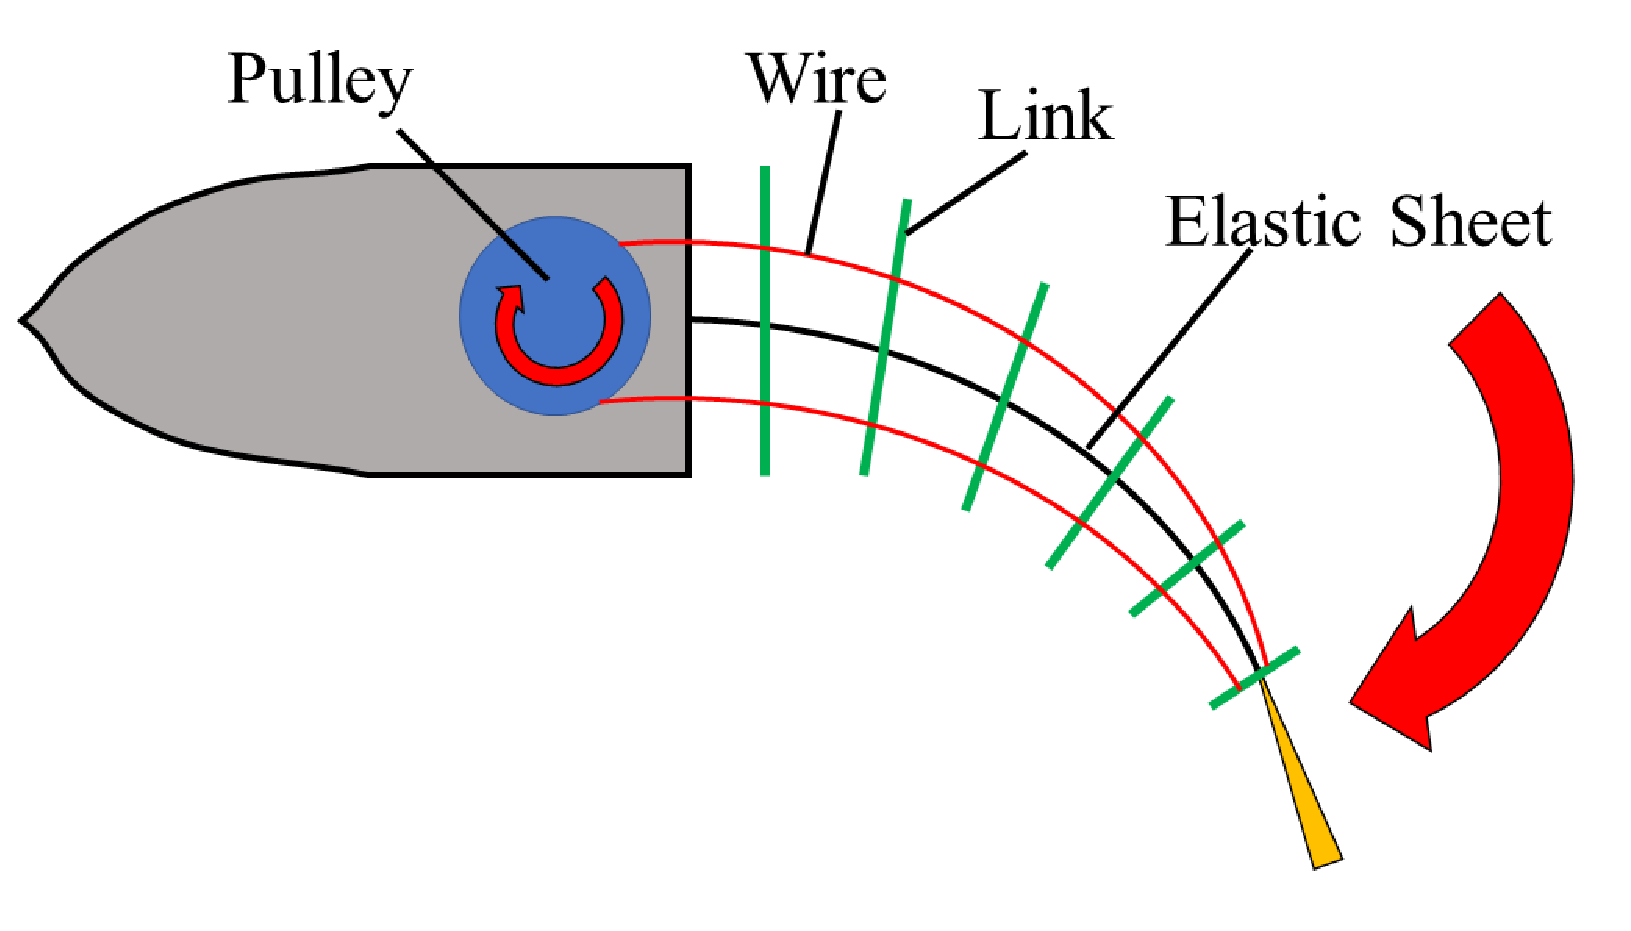
\includegraphics[width=0.7\linewidth]{/Users/watanabe_shouta/2024_graduation_thesis/picture/waiyakudou.eps}
   \caption{ワイヤ駆動のイメージ}
   \label{fig:waiyakudou}
\end{figure}
\noindent の二つのLi-ionバッテリーを使用している.そのため,頭部は防水が必要となり,頭部の断面にOリングをはめ込むことによって防水を行っている.
頭部はネジ穴が空いたものと,ナット用の穴が空いたものに分かれており,これらはM1.7ネジで固定される.

胴体部は骨格リンク(PLA樹脂)と弾性体(ポリプロピレン板,厚さ0.75 mm),尾びれ(TPU樹脂,厚さ2 mm)で構成されており,骨格リンクは図のように楕円形にして作製し,ワイヤを通す穴を空けている.
\begin{figure}[htbp]
    \centering
    \includegraphics[width=0.80\linewidth]{/Users/watanabe_shouta/2024_graduation_thesis/picture/sisaku.jpg}
    \caption{試作機の外観}
    \label{fig:sisaku}
\end{figure}
\begin{figure}[htbp]
    \centering
    \includegraphics[width=0.80\linewidth]{/Users/watanabe_shouta/2024_graduation_thesis/picture/tentativeschematic.png}
    \caption{試作機の構造}
    \label{fig:kouzou_sisaku}
\end{figure}
\begin{figure}[H]
    \centering
     \begin{minipage}[b]{0.50\linewidth}
        \centering
        \setPicture{ring.jpg}
        \caption{頭部断面のようす}
        \label{fig:danmen}
     \end{minipage}
     \hspace{0.05\linewidth}
     \begin{minipage}[b]{0.25\linewidth}
        \centering
        \setPicture{jikkilink.png}
        \caption{骨格リンク}
        \label{fig:link_sen}
     \end{minipage}
\end{figure}

\begin{figure}[t]
    \centering
    \setPicture{sisakuoyogu2.png}
    \caption{遊泳テストの様子}
    \label{fig:test_sisaku}
\end{figure}

ロボット作製後,遊泳テストを行った(図\ref{fig:test_sisaku}).

\subsubsection{試作機から得られた知見}
試作機の作製・動作確認を通して得られたこととして,まず頭部をネジとOリングを用いて防水する方法は限度があることが分かった.ネジの締め方や締め具合を何度か調整しても
図のように頭部下方は浸水してしまい,完全な防水機能を有することはできていなかった.また,頭部を固定するネジが多いと,バッテリー交換がしにくく,メンテナンス性が
悪くなるということも分かった.以上のことから防水方法を変更し,メンテナンス性を向上させた頭部に改良することが必要だとわかった.

\subsection{ワイヤ駆動式柔軟外皮装着型魚ロボットの開発}
ここからは本研究で開発した機体について述べる.
図に開発した機体の外観を,図に構造を示す.開発した魚ロボットは体長470 mm,重量は重りを含めて710 gである.ロボットの外形は先行研究において作製されたアジのモデルデータをもとに作製し,
サイズは2倍とした本機体は頭部・胴体部・外皮の3つからなり,頭部と胴体部をそれぞれ別の柔軟外皮で包む構造になっている.
\subsubsection{頭部}